\chapter{Results}
In this section we present and compare results of the four models aplied in STLF. The performance of the models are evaluated using MAPE, MAE, RMSE and R\^2. These metrics can give us a clear picture and comparisons framework for each of the model performance.  The goal is to represent the accuracy, robustness and suitability of the ML and AI models to solve STLF.

The metrics theory is explained in \ref{sec:eval_metrics} which shows the mathematics behind each of the metrics used in the research. The methodology shows the creation of the models and how these results were produced. 


\subsubsection{Dataset Results}
 The continuous\_dataset.csv contained well ordered data that was collected with minimum errors, empty data was filled using the forward and back-filling process.Figure \ref{fig:originaldataset}
 \begin{figure}[h]
 	\centering
 \begin{minipage}[b]{0.45\linewidth}
 	\centering
 	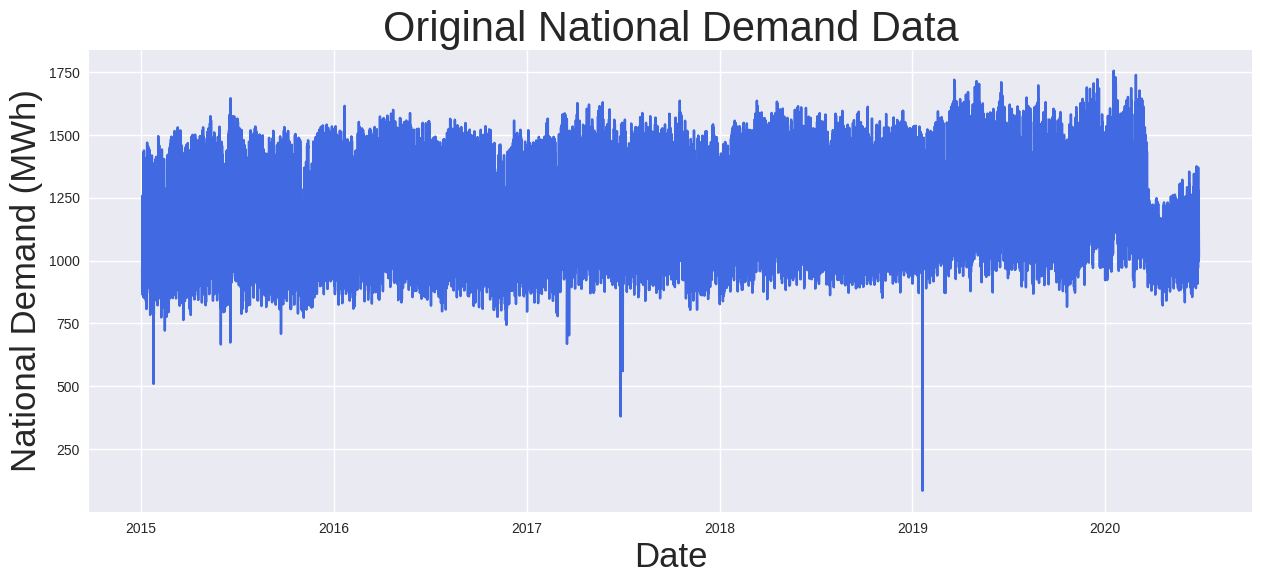
\includegraphics[width=\linewidth]{Chapters/images/results/original_dataset}
 	\caption{The original national demand .}
 	\label{fig:originaldataset}
 \end{minipage}
 \begin{minipage}[b]{0.45\linewidth}
 	\centering
 	\includegraphics[width=\linewidth]{"Chapters/images/results/train test split_after HI"}
 	\caption{HI processed dataset with traintest split.}
 	\label{fig:train-test-splitafter-hi}
 \end{minipage}
 \end{figure}
 
 The HI method explained in section \ref{sec:HI_method}, was used to handle outliers in the dataset, fixing all data-points that deviated from the normalcy presented in the dataset. After the implementation of the HI-method the train test split of 80/20 was implemented. Figure \ref{fig:train-test-splitafter-hi} shows the effectiveness of the HI method in removing noisy details in the dataset.

 \begin{figure}[h]
  	\centering
  	% First figure
  	\begin{minipage}[b]{0.45\linewidth}
  		\centering
  		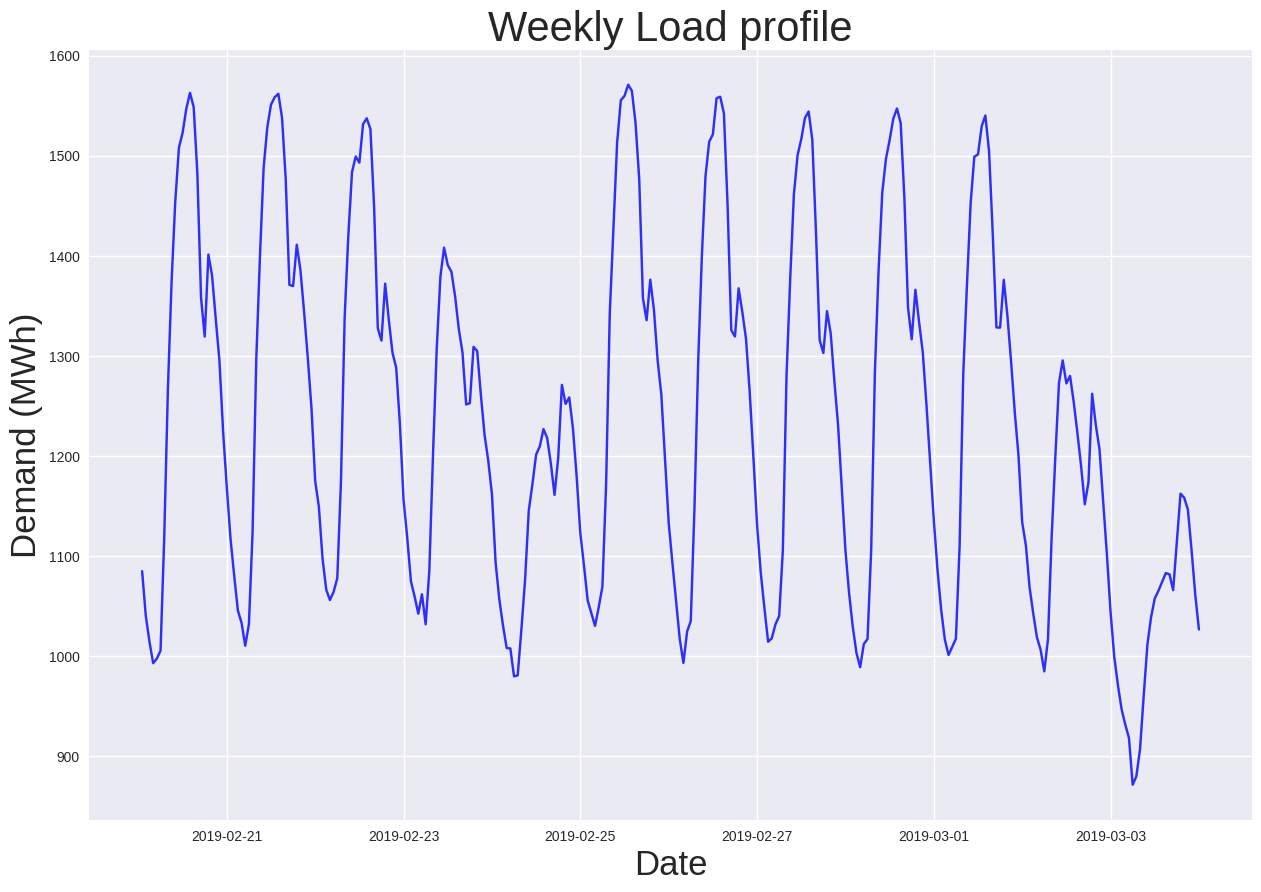
\includegraphics[width=\linewidth]{Chapters/images/results/weekly_load_profile.png}
  		\caption{The general weekly national load profile.}
  		\label{fig:weeklyloadprofile}
  	\end{minipage}
  	\hfill
  	% Second figure
  	\begin{minipage}[b]{0.45\linewidth}
  		\centering
  		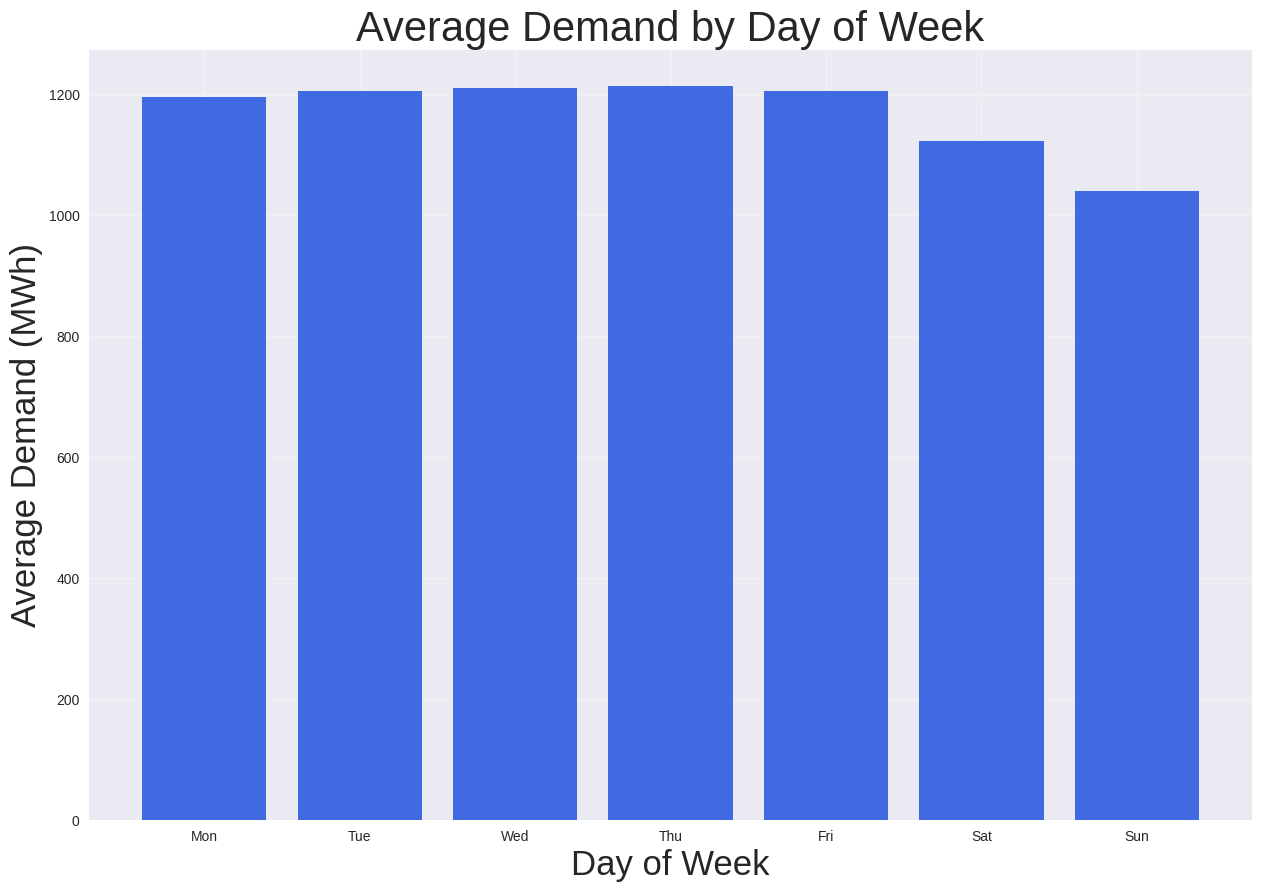
\includegraphics[width=\linewidth]{Chapters/images/results/average_daily_demand.png}
  		\caption{The weekly average daily demand }
  		\label{fig:averagedailydemand}
  	\end{minipage}
  \end{figure}
  
  
  To further understand the dataset, it was broken down to give the more insight on how the data and load behaves at different points. Firstly the weekly load profile in figure \ref{fig:weeklyloadprofile} shows a daily pattern that the load exhibits.The trend shows a higher usage during the week and lower usage in the weekend, with the lowest usage day being Sunday. 
  
  
  Figure \ref{fig:averagedailydemand} shows the average daily demand  of electricity. It also shows a higher usage during the week and lower consumption on the weekend, with Sunday being the lowest consumption day. 
  \begin{figure}[h]
  	\centering
  	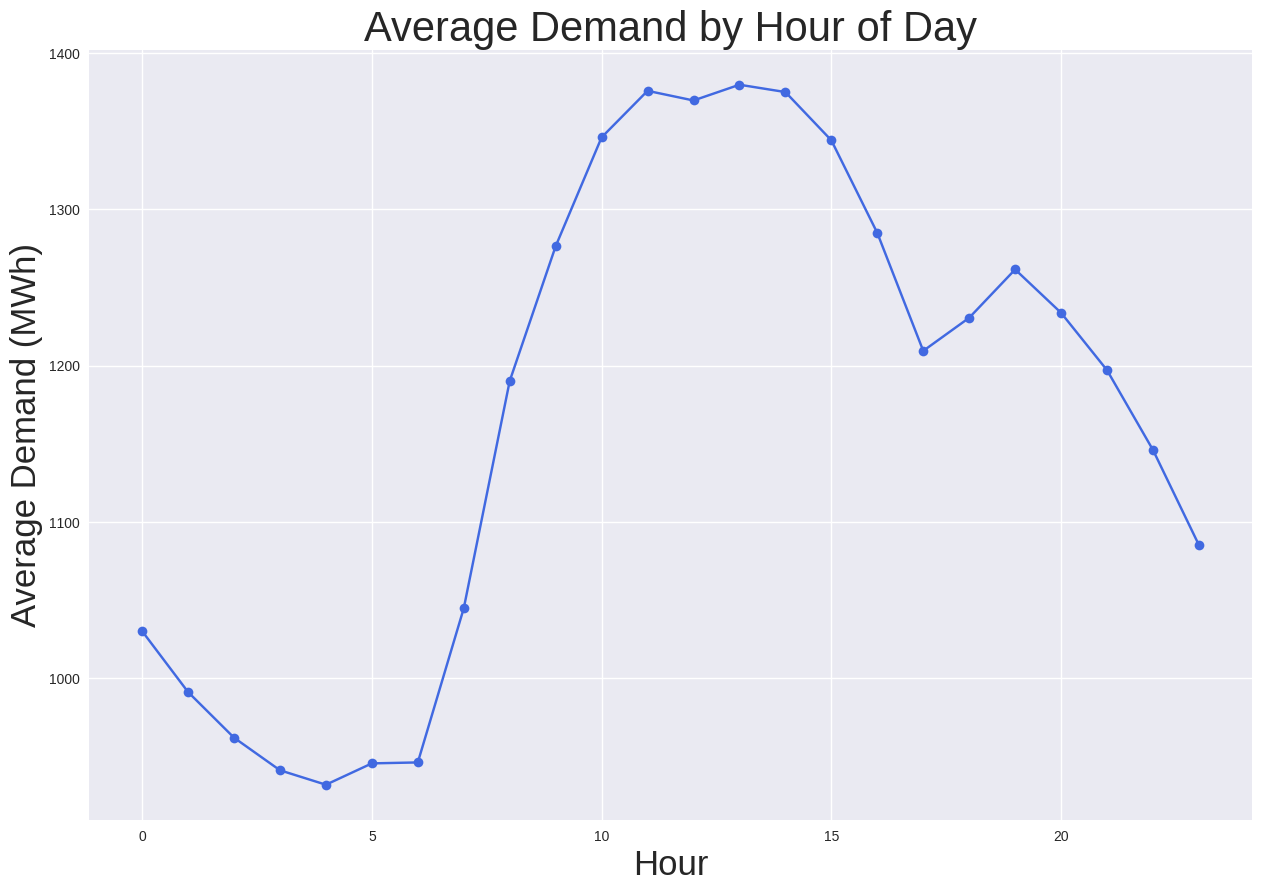
\includegraphics[width=0.45\linewidth]{Chapters/images/results/average_hourly_demand}
  	\caption{Average hourly demand of electricity between 2015 and 2020 in panama}
  	\label{fig:averagehourlydemand}
  \end{figure}
  
  Figure \ref{fig:averagehourlydemand} shows the average hourly usage of data. The averages show that the lowest consumption is in the early hours of the day, with a steady rise in the early morning leading to a peak at midday. After midday there is a steady decrease in demand with a slight increase between the 18th and 20th hour of the day, this is followed by a drop in usage leading to the early hours of the day.  


\subsubsection{Model Results}